\section{Data Description}

Obtaining the heterogenous data can be challenging, especially when an EHR dataset is involved \cite{wang2021EHRa}. The data acquisition involves multiple steps. The first step is to obtain both geospatial boundaries and EHR data that match one another. The second step is to pre-process the EHR data to remove empty and erroneous values. The final step is to transform the data into a format that is suitable for cartograms.

\subsection{Geospatial Data}

Geospatial boundaries, or shapefiles, were obtained from the sources described below.
{
\begin{figure}[tb!]
    \centering
    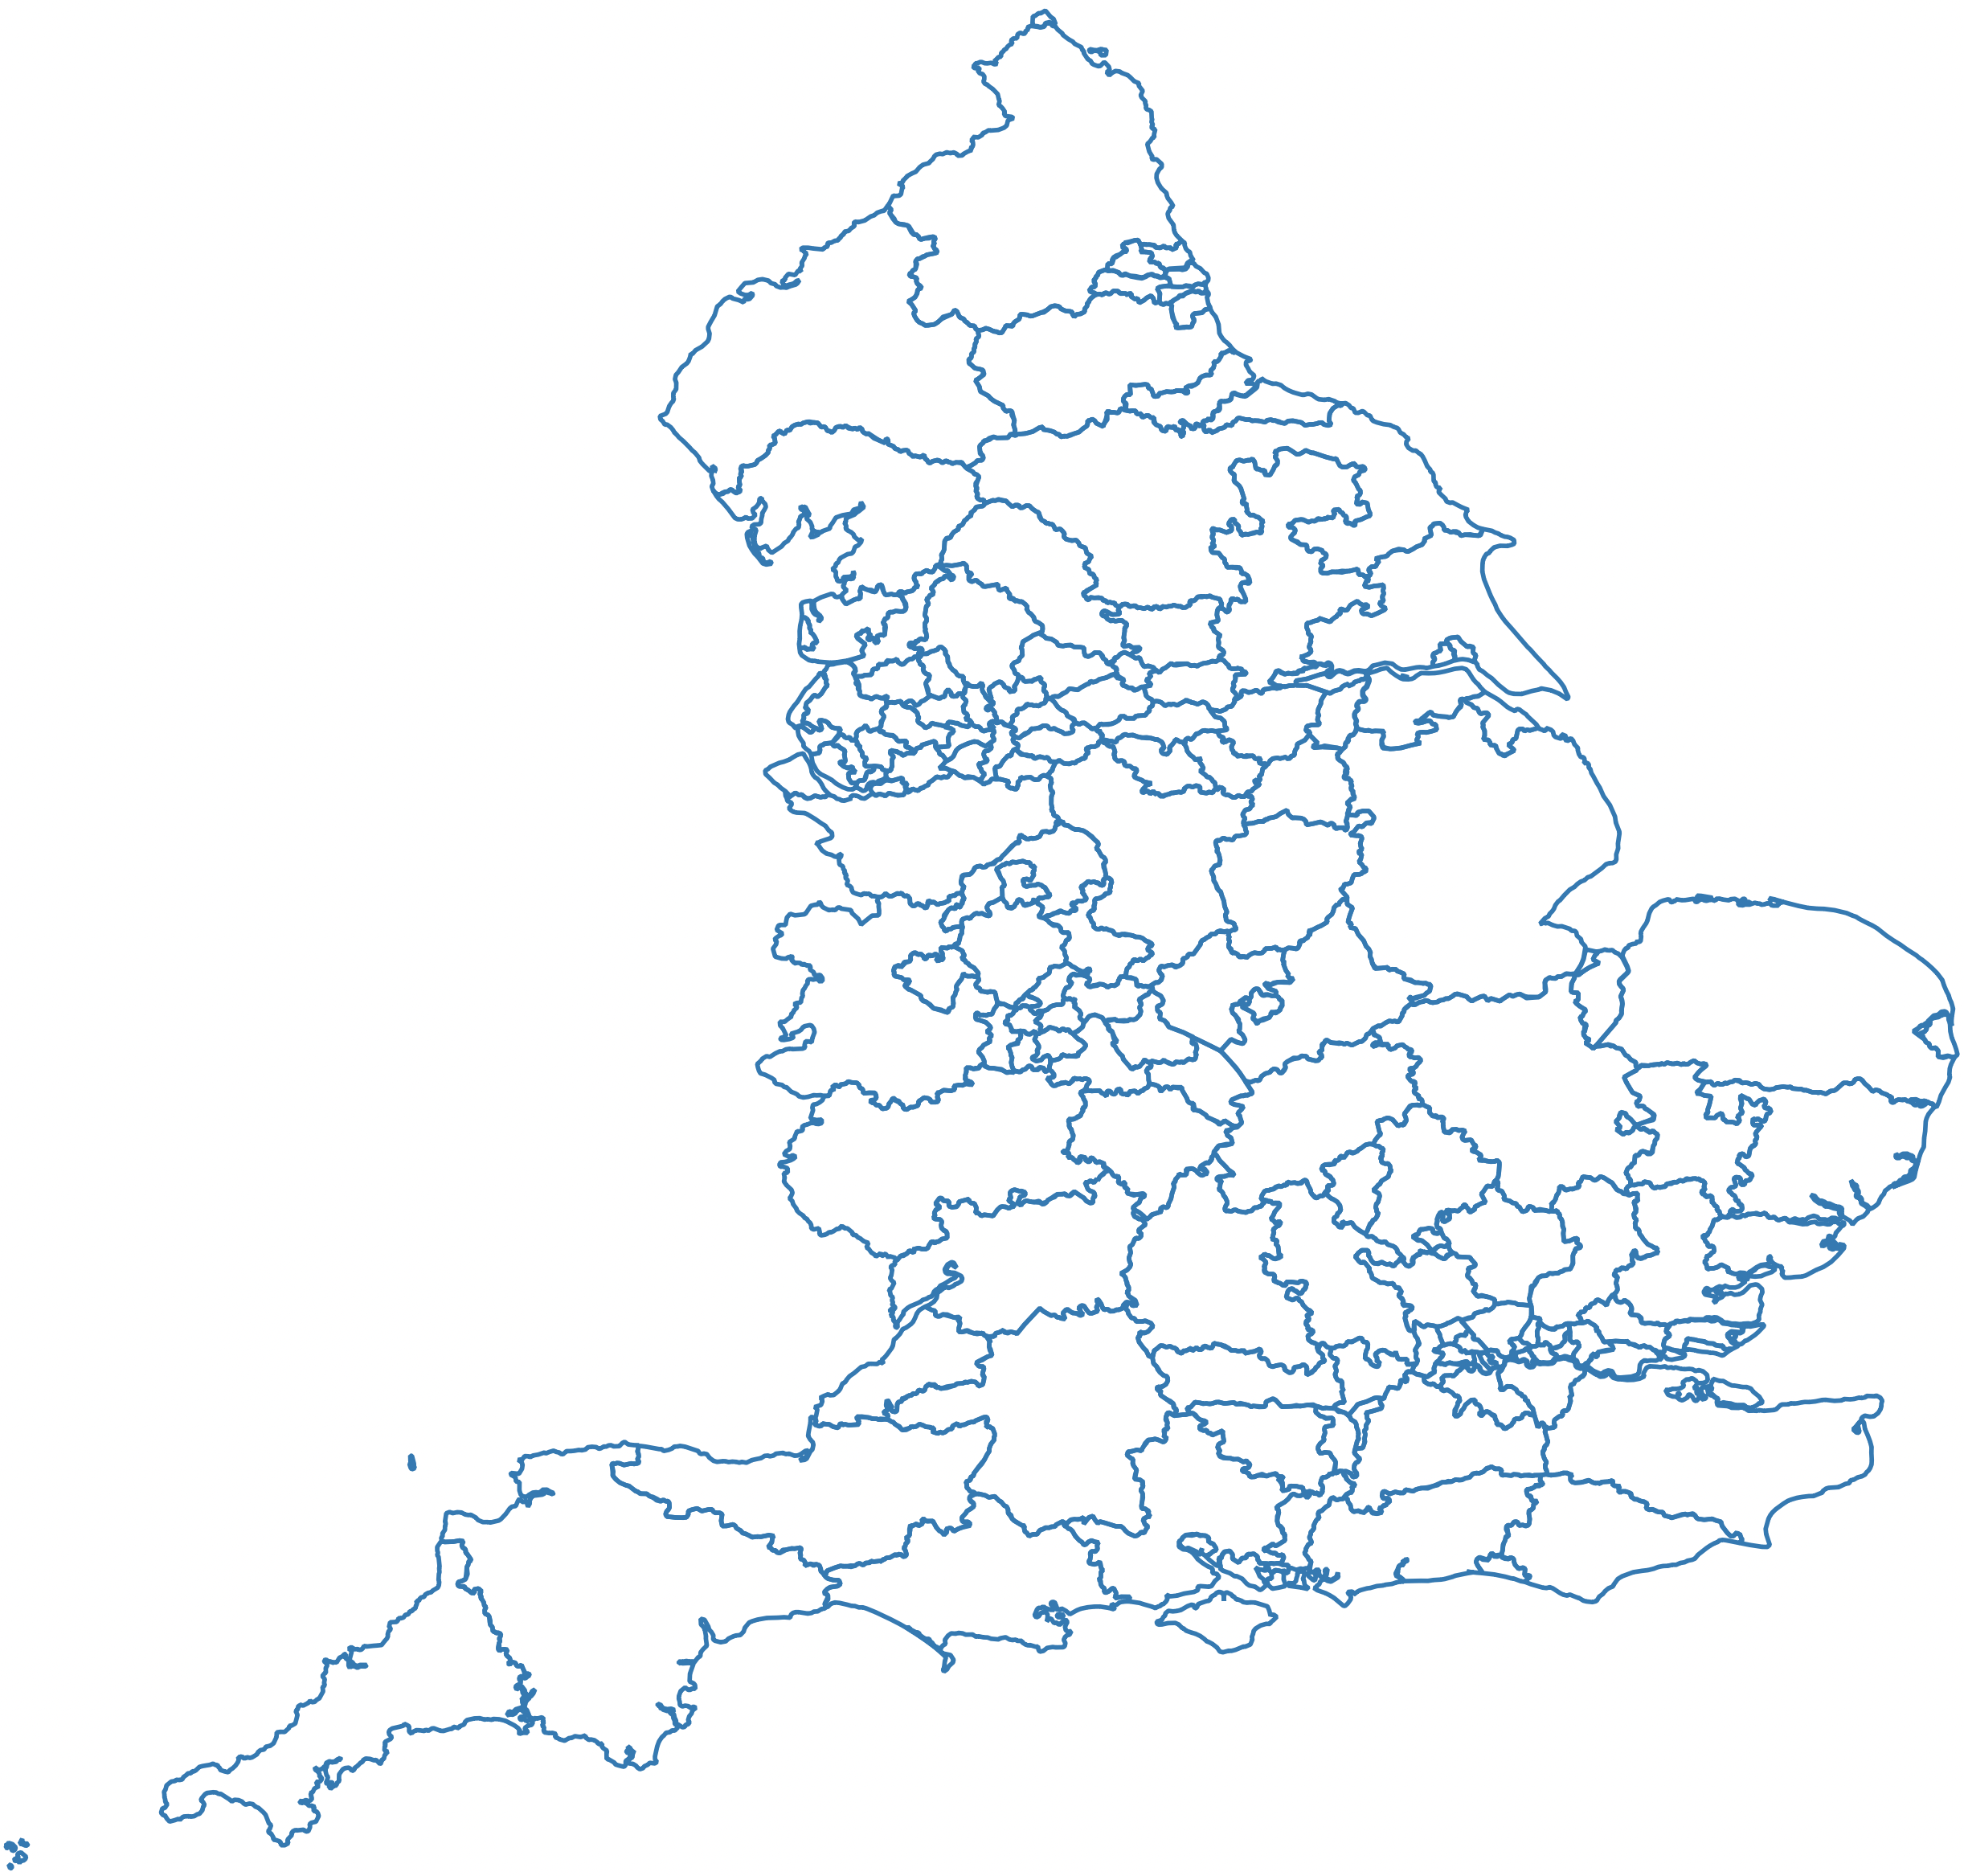
\includegraphics[width=0.6\columnwidth]{figure/ccg.png}
    \caption{A map of 135 CCGs in England as of 2020, obtained from the Open Geography portalx \cite{opengeographyportalxOpen}.}
    \label{fig:ccg}
\end{figure}
}

\bobgraph{Clinical Commissioning Groups Shapefile}

Clinical Commissioning Groups (CCGs) are the primary administrative and geographic unit of the National Health Service (NHS) in the UK \cite{nhsNHS}. The number of CCGs changes over time due to the NHS re-organization. The most up-to-date shapefile is available from the Open Geography portalx \cite{opengeographyportalxOpen}. We decided to use the CCG shapefile from 2020 at the time of writing, because there is still no public EHR data published based on the latest CCG re-organization that took place in 2021.

\bobgraph{River Features}

We used OpenStreetMap \cite{openstreetmapRelation} as our data source to obtain shapefiles for River Thames, River Trent and River Great Ouse in England. These rivers were chosen as they are well-known rivers and pass through regions with dense population, and provide informative geographical and topological cues. 

We first obtain a relation ID by searching for a river, e.g. River Thames, on OpenStreetMap. The relation ID is used to construct a query (See Listing~\ref{overpass}) which enables the user to download the entire river shapefile using Overpass Turbo \cite{overpassturboOverpass}.

\begin{lstlisting}[caption={The query that downloads the shapefile of River Thames from OpenStreetMap via the Overpass Turbo API.}, label={overpass},captionpos=b]
    relation(2263653);>>;
    out skel;
\end{lstlisting}

After acquiring the shapefiles, we used QGIS \cite{qgisWelcome} to manually adjust projections and scales, and merge them into one shapefile. Finally, mapshaper \cite{blochMapshaper} is used to convert the merged shapefile into a TopoJSON \cite{TopoJSON} file. TopoJSON eliminates redundant coordinates in the data, this improves the rendering speed of our implementation.

\subsection{EHR Data}

We obtained the Clinical Commissioning Group Outcomes Indicator Set (CCG OIS) from NHS Digital \cite{nhsdigitalClinical}. The OIS is a set of indicators that are used to measure the quality of care and the associated health outcomes in the NHS. Some datasets include:
\begin{itemize}
    \item Under 75 mortality
    \begin{multicols}{2}
        \begin{itemize}
            \item Cardiovascular disease
            \item Respiratory disease
            \item Liver disease
            \item Cancer
        \end{itemize}
    \end{multicols}
    \item Emergency hospital admission
        \begin{itemize}
            \item Stroke
            \item Alcohol-specific admission and readmission
            \item Coronary heart disease
            \item Readmissions within 30 days of discharge
            \item Children with lower respiratory tract infections
        \end{itemize}
\end{itemize}

For all datasets, a spreadsheet including the following data is provided:

\begin{itemize}
    \item Reporting period: Calendar year of registration
    \item Period of coverage: Start and end date or reporting period
    \item Breakdown: Organization type
    \item ONS code: UK Office for National Statistics CCG code
    \item Level: CCG Code
    \item Level description: CCG Name
    \item Gender
    \item Indicator value: Directly standardized mortality rate
    \item CI lower: lower 95\% confidence interval
    \item CI upper: upper 95\% confidence interval
    \item Denominator: The count of registered patients
    \item Numerator: Number of deaths
\end{itemize}

Each CCG has a unique ONS code, which is used to link the CCG shapefile with the statistical data.